\documentclass{report}
\usepackage{float}

% for the image in the title
\usepackage{tikz}

% custom spacing
\usepackage{setspace}
\onehalfspacing

% footer and header
\usepackage{fancyhdr}
% \setlength{\headheight}{15.2pt}

% underlining
\usepackage{ulem}


% Table of contents link to corresponding sections
\usepackage{hyperref}
\hypersetup{
	colorlinks,
	citecolor=black,
	filecolor=black,
	linkcolor=black,
	urlcolor=black
}

\usepackage{amsmath}
% Remove che "Chapter" string before chapters
\iffalse
\makeatletter
\def\@makechapterhead#1{%
	\vspace*{50\p@}%
	{\parindent \z@ \raggedright \normalfont
		\interlinepenalty\@M
		\Huge\bfseries  \thechapter.\quad #1\par\nobreak
		\vskip 40\p@
}}
\makeatother
\fi

% Fancy chapters
\usepackage[Bjarne]{fncychap}
% options: Sonny, Lenny, Glenn, Conny, Rejne, Bjarne, Bjornstrup

\begin{document}
	
	
	%title page
	\begin{titlepage}
		\begin{figure}[t]
			\centering
\includegraphics[width=0.3\textwidth]{images/unitn-logo}
		\end{figure}
		\begin{center}
			\textsc{ \LARGE{Università degli Studi di Trento \\}}
			\textsc{ \LARGE{Facoltà di Informatica\\ }}
			\textnormal{ \LARGE{Corso di Ingegneria del Software\\}}
			\vspace{30mm}
			\fontsize{10mm}{7mm}\selectfont 
			\textup{Fix Mi \\ Application Implementation and Documentation}\\
		\end{center}
		
		\vspace{25mm}
		
		\centering
		\large Gruppo G43: \\ Giovanni Santini\\ Riginel Ungureanu \\ Valerio Asaro
		
		\vspace{20mm}
		
		\centering{\large{Anno Accademico 2023/2024 \\ Trento }}
		
	\end{titlepage}
	
	
	
	
	% use header and footers
	\pagestyle{fancy}
	\fancyhead[R]{\chaptername\ \thechapter}  % header
	
	%\maketitle
	\tableofcontents
	\newpage
	
	
	
	\section{Scopo del documento}
	
	
	\section{Implementazioni}
	
	\section{Informazioni del Documento}
	
	% table
	\begin{center} % center the table
		\centering
		\begin{tabular}{ |p{4cm}|p{4cm}|  }
			\hline
			\centering Campo & \qquad\qquad Valore \\ % I found no other way...
			\hline
			Titolo del Documento & Application Implementation and Documentation \\
			\hline
			Titolo del Progetto & Fix Mi \\
			\hline
			Autori del Documento &
			Giovanni Santini \\ & Riginel Ungureanu \\ & Valerio Asaro \\
			\hline
			Amministratore Progetto & Riginel Ungureanu\\
			\hline
			Versione del documento & 1.0 \\
			\hline
		\end{tabular}
	\end{center}
	
	
	
\chapter{Backend}

Il seguente capitolo descrive l'implementazione, con il supporto di diagrammi "UML" e codice, della parte "Backend" dell'applicazione, in riferimento a quanto detto nei precedenti documenti quali "Analisi dei Requisiti", "Specifica dei Requisiti" e del "Documento di Architettura".  Il capitolo è strutturato partendo da una visione generale dell'infrastruttura, andando verso una visione più specifica e dettagliata.


Gli estratti di codice verranno mostrati nel seguente formato:
\begin{figure}[H]
	\centering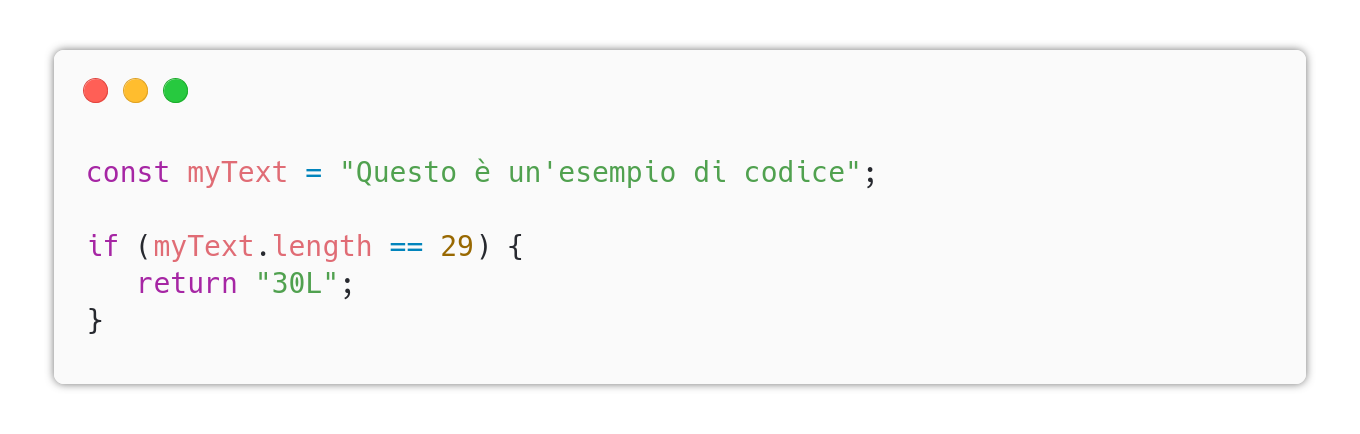
\includegraphics[width=1\textwidth]{images/example_code_01.png}
	Esempio di estratto di codice
\end{figure}

\subsection*{Tecnologie}

In questo capitolo verranno menzionate più volte alcune tecnologie, dunque ne viene riportata una breve descrizionee sotto:
\begin{itemize}
	\item "Docker": tecnologia che raccoglie il software in unità standardizzate chiamate container, offrendo tutto il necessario per la loro corretta esecuzione, incluse librerie, strumenti di sistema, codice e runtime. Il logo ricorda una balena di colore azzurro con dei rettangoli al di sopra rappresentanti dei containers, come se la balena stessa fosse una nave.
	\item "Docker Compose": software per la gestione di molteplici docker containers contemporaneamente. L'icona rappresenta un polpo con dei parallelepipedi azzurri tra i tentacoli.
	\item "Nginx": intermediario tra le richieste da parte dei client e il server. Può essere usato come load balancer, cache o proxy. Il logo è raffigurato da un N bianca con sfondo verde.
	\item "MongoDB": DBMS non relazionale. Il logo rappresenta una foglia verde.
	\item "Express": framework backend per applicazioni web in javascript. Il logo è formato dalle due lettere "e" e "x" in nero.
	\item "React": framework frontend lo sviluppo di applicazioni web. L'icona ricorda un atomo.
\end{itemize}

\section{Architettura dei Microservizi}

L'architettura proposta si basa sulla divisione logica (e fisica) delle funzionalità dell'applicazione tramite la distinzione di \textit{Microservizi}. Ciascun microservizio è indipendente dagli altri ed è composto a sua volta da una frontend e una backend distinte. Per tale ragione, è più accurato parlare di micro-frontend e micro-backend.

\subsection*{Vantaggi di un'architettura basata su microservizi}

Da un punto di vista di sviluppo, un'architettura non monolitica permette lo sviluppo asincrono dei singoli microservizi, oltre a facilitare la divisione del lavoro nelle varie parti. Tale architettura ha anche dei vantaggi a livello di performance in quanto il carico di lavoro chel'applicazione processa viene distribuito su più processi diminuendo il carico sul singolo. Altri vantaggi sono la scalarità dia una componente dell'applicazione in base alle esigenze e la ridondanza in quanto possono esistere più istanze di un microservizio contemporaneamente.

\subsection*{Svantaggi}

Un'architettura a microservizi è intrinsecamente più complessa nella progettazzione e nella menutenzione rispetto ad una architettura tradizionale. La necessità di orchestrare e mettere in comunicazione i diversi microservizi richiede particolari accortezze nella parte di design e di deploy. Tali problematiche sono state valutate con cura dal team di sviluppo.

\section{Visione Generale}
Prima di analizzare il singolo microservizio, questa sezione illustra una visione generale dell'applicazione e degli strumenti utilizzati per la realizzazione dell'infrastruttura, per poi concentrarsi sulle parti comuni di ogni microservizio e infine sul singolo microservizio.


\subsection*{Infrastruttura}

Si presti attenzione alla seguente infografica dell'infrastruttura implementata:

\begin{figure}[H]
	\centering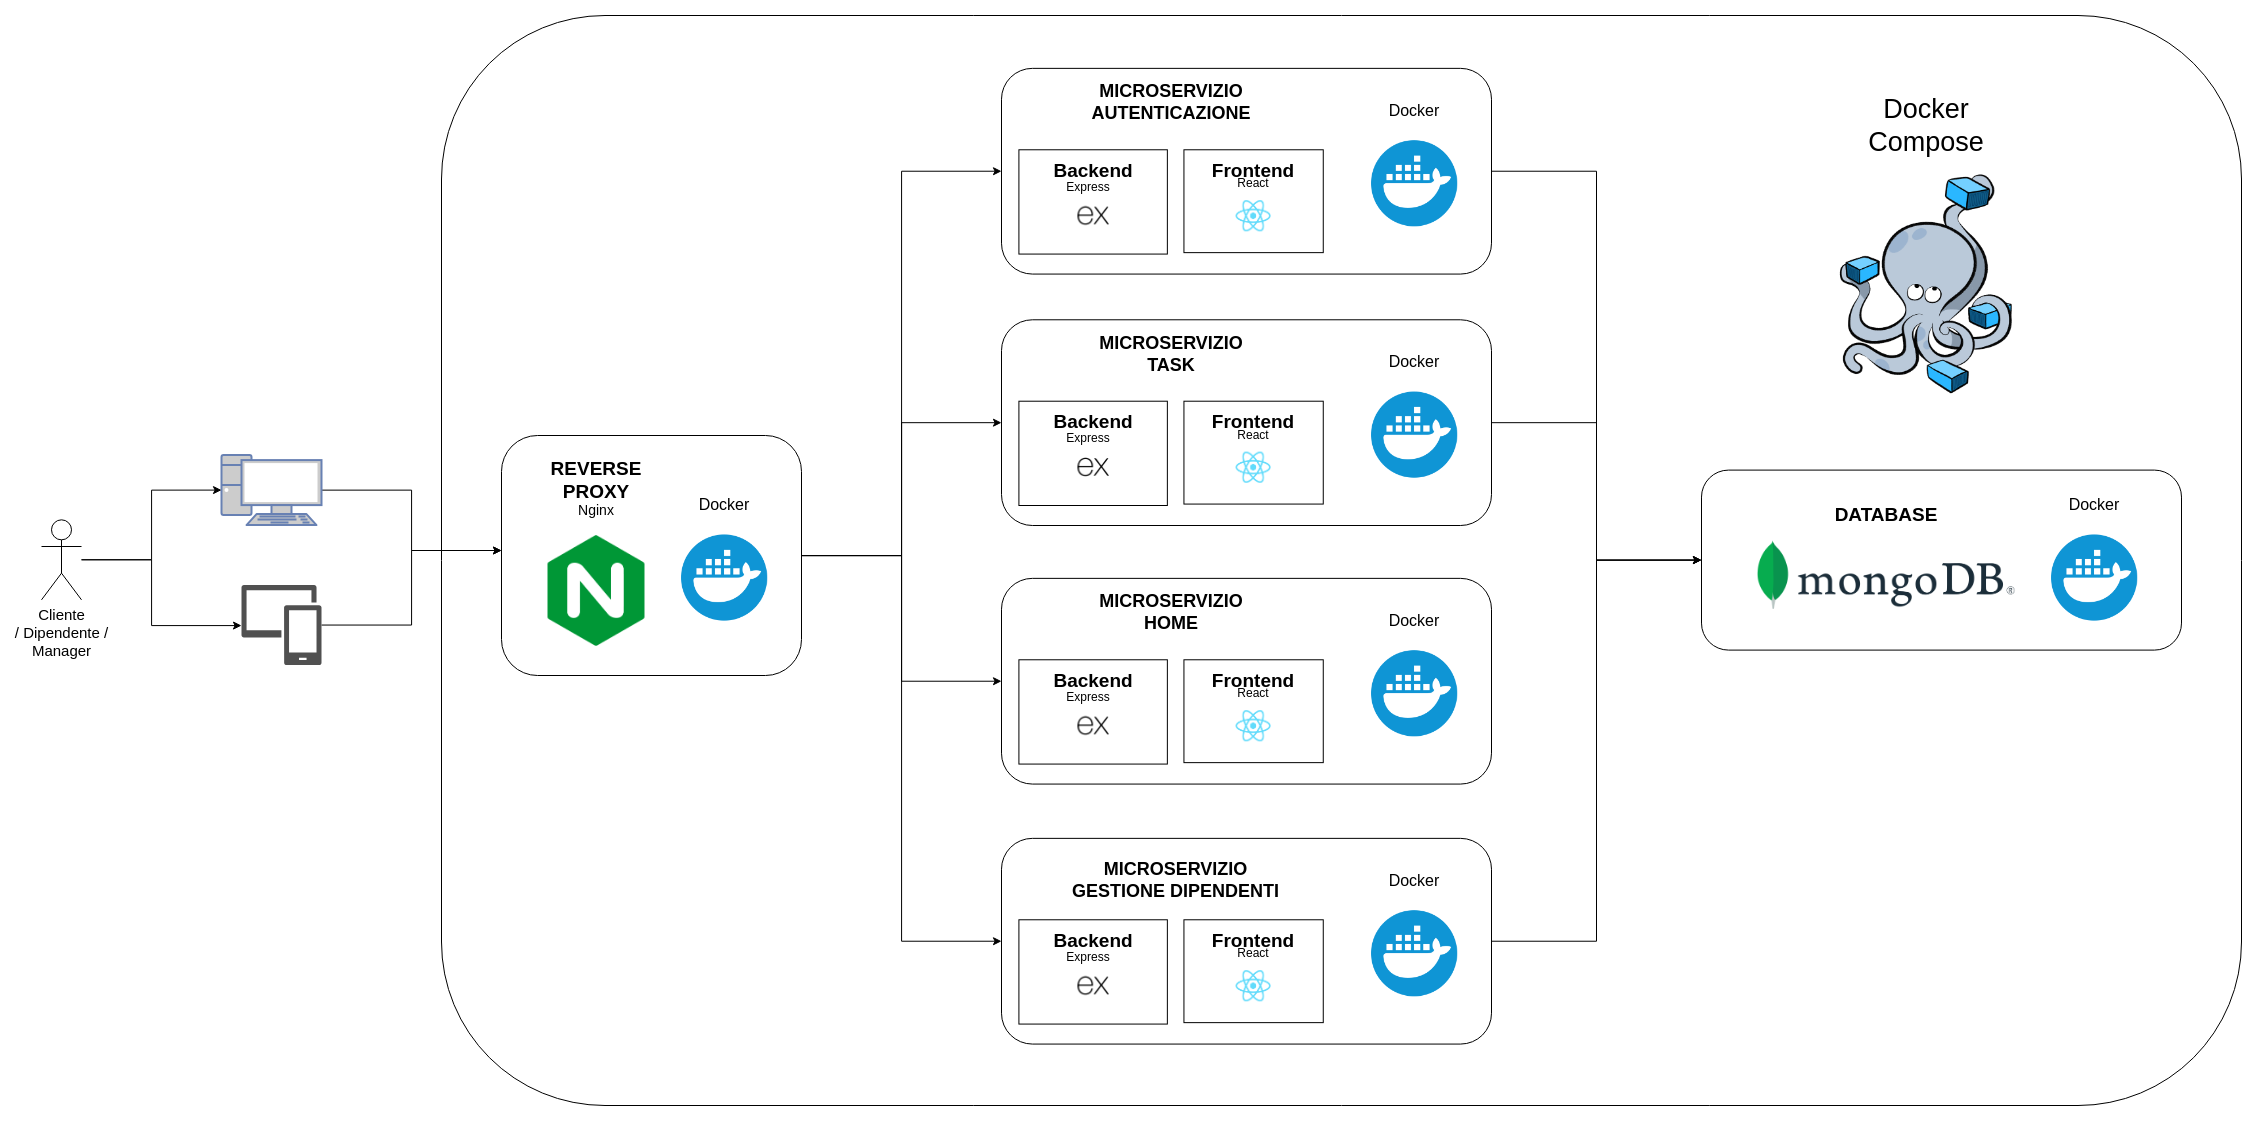
\includegraphics[width=1\textwidth]{images/diagramma_microservizi.png}
	Schema dei microservizi
\end{figure}

L'intera infrastruttura viene inizializzata con \textit{Docker Compose}. In particolare, \textit{Docker Compose} si occupa di impostare i containers sullo stesso network con un IP statico e impostare le variabili di ambiente come le porte e gli IP dei rispettivi microservizi, oltre ad inizializzare i containers, le porte e volumi condivisi.

Se eseguito su un singolo host, il network di default segue la seguente struttura:
\begin{figure}[H]
	\centering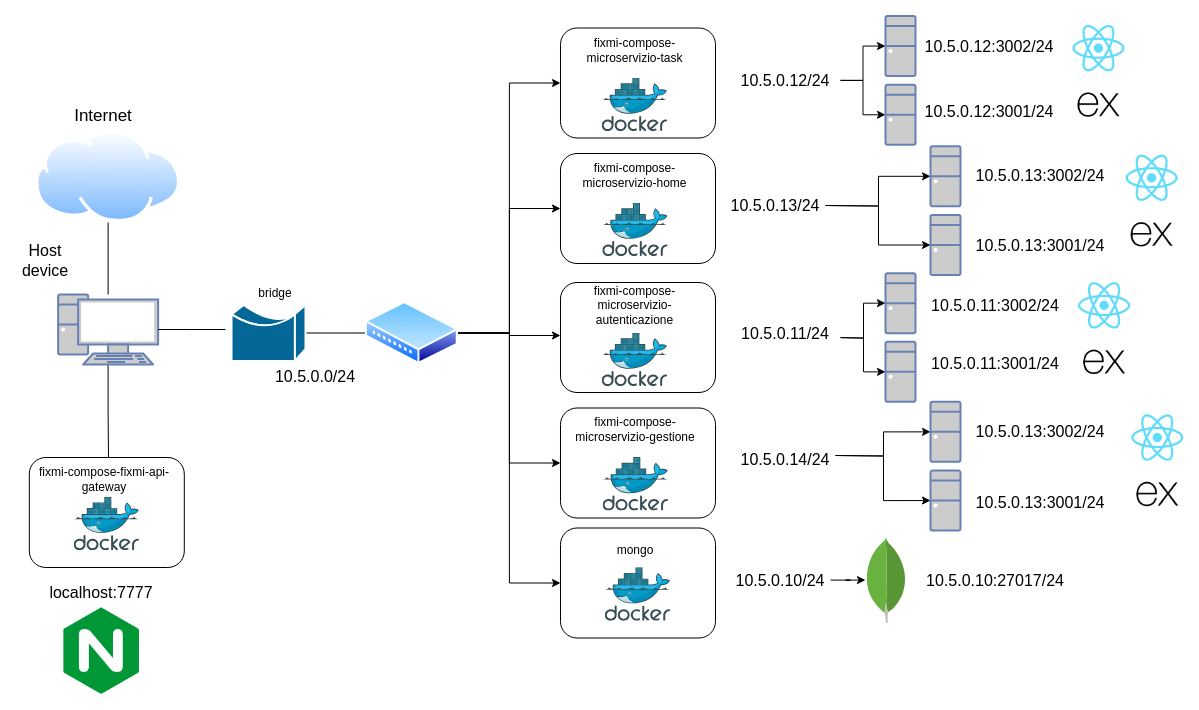
\includegraphics[width=1\textwidth]{images/network.png}
	Schema del network dei microservizi
\end{figure}

Docker imposta i microservizi sul network 10.5.0.0/24 con i seguenti IP:
\begin{itemize}
	\item "MongoDB": 10.5.0.10/24
	\item "Microservizio Autenticazione": 10.5.0.11/24
	\item "Microservizio Task": 10.5.0.12/24
	\item "Microservizio Home": 10.5.0.13/24
	\item "Microservizio Gestione Dipendenti": 10.5.0.14/24
	\item "Reverse Proxy": localhost
\end{itemize}

Per ogni servizio all'interno dei containers sono state assegnate le seguenti porte:
\begin{itemize}
	\item "Backend": 3001
	\item "Frontend": 3002
	\item "MongoDB": 27017
	\item "Reverse Proxy": 7777
\end{itemize}

Due microservizi particolari sono il database e il reverse proxy. Il database fornisce la possibilità di salvare in modo permanente i dati dell'applicazione, mentre il reverse proxy permette di accedere facilmente all'ip di un microservizio attraverso una mappatura di ip. I software scelti sono rispettivamente \textit{MongoDB} e \textit{Nginx}.

In particolare, \textit{Nginx} associa i path nel seguente modo:
\begin{figure}[H]
	\centering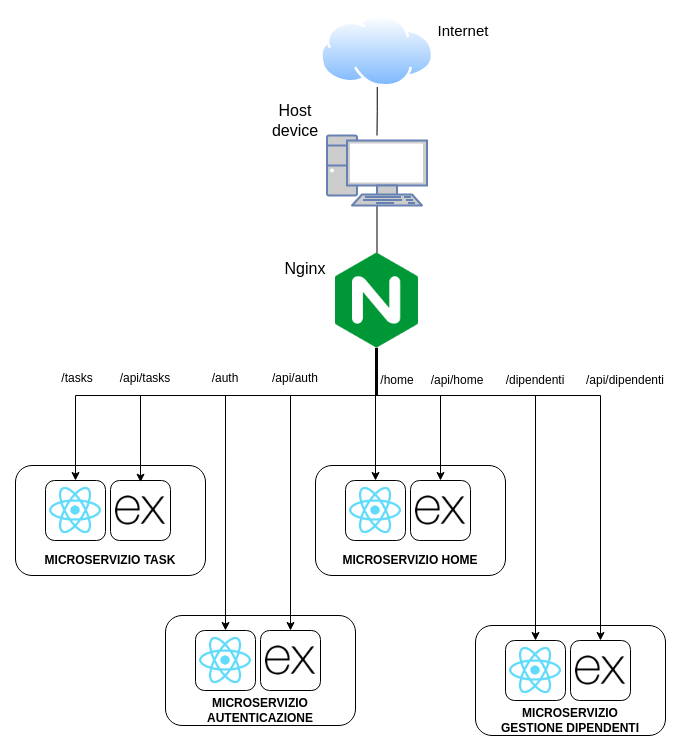
\includegraphics[width=1\textwidth]{images/nginx.png}
	Schema delle routes di Nginx
\end{figure}

\subsection*{Codice: docker-compose.yaml}

Si prenda come esempio questo frammento di codice per la definizione del microservizio task:
\begin{figure}[H]
	\centering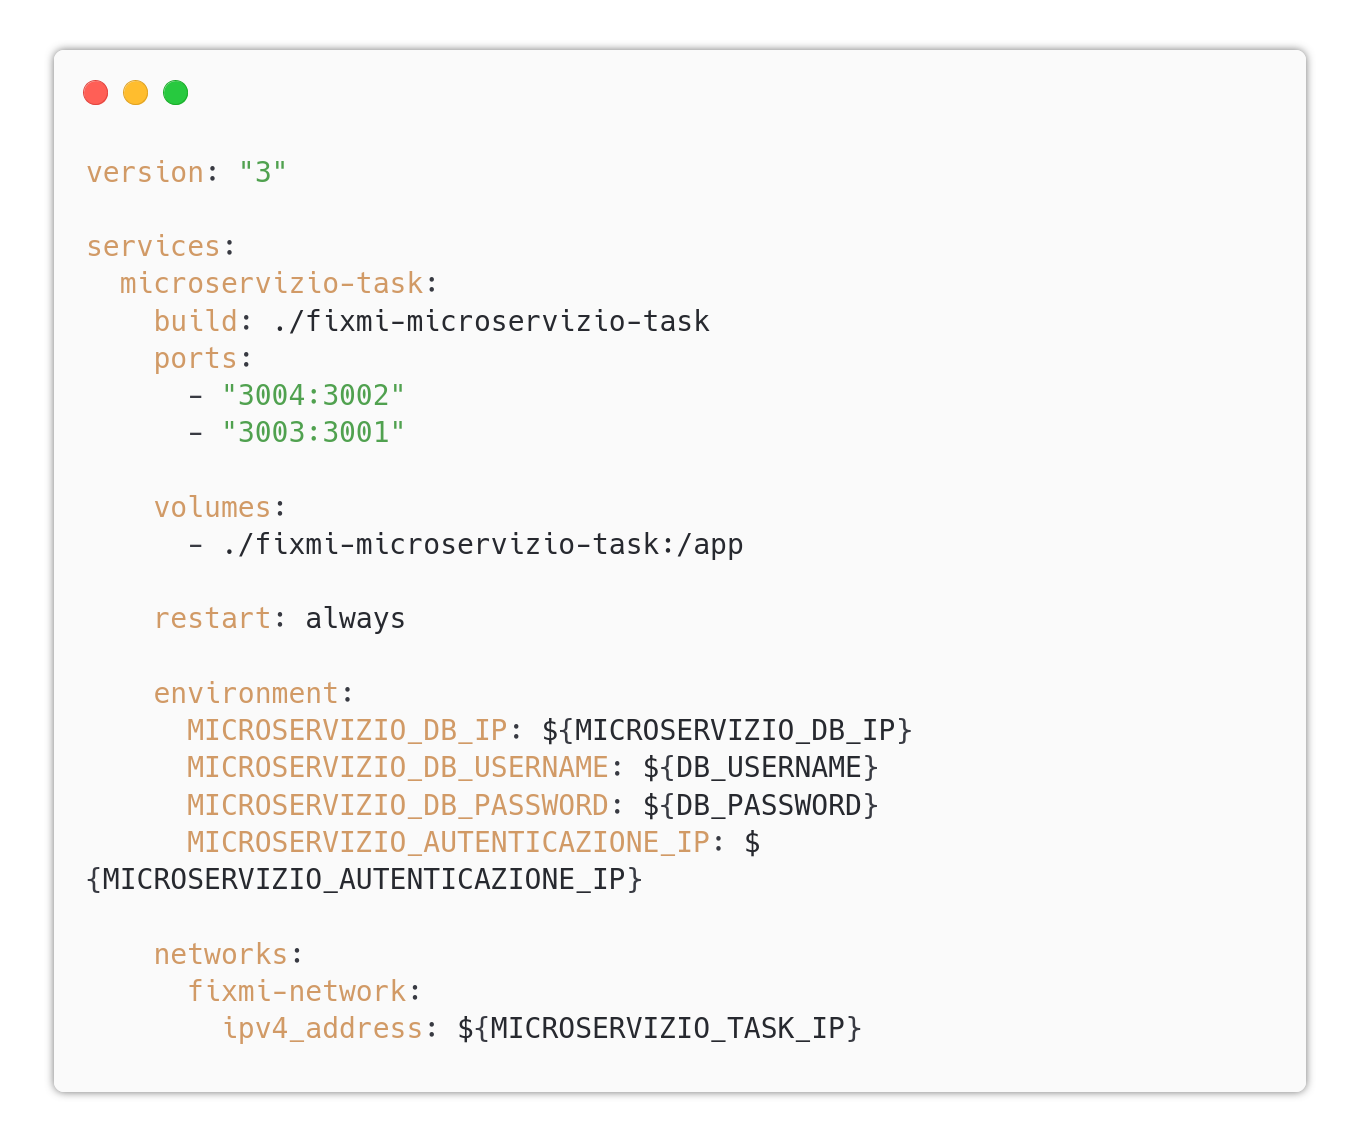
\includegraphics[width=1\textwidth]{images/docker_code_01.png}
	Estratto dal file "docker-compose.yaml"
\end{figure}

In questo codice, notiamo che le porte vengono impostate sotto la sezione "ports", così come i volumi e il network. Le variabili d'ambiente contenenti i vari ip e le credenziali del database sono contenute nel file ".env" presente nella radice della cartella.

\subsection*{Codice: nginx.conf}



\section{Parti comuni ad ogni microservizio}

\subsection{Scelta del Linguaggio}

\subsection{Frameworks e Dipendenze}



\section{Microservizio Autenticazione}

\section{Microservizio Task}

\section{Microservizio Gestione Dipendenti}

\section{Microservizio Home}

\chapter{Frontend}

	
\end{document}